\documentclass{article}[18pt]
\usepackage{../../../../format}
\usepackage{tabularx}
\lhead{Computational Thinking - Rob Powell}


\begin{document}
\begin{center}
\underline{\huge What is computer hardware?}
\end{center}
\section{PC Internals}
Motherboard:
\begin{itemize}
\item CPU Socket
\item RAM Slots (Memory, temporary storage)
\item Northbridge Chipset - Communication between fast components (CPU, Graphics, RAM)
\item Southbridge Chipset - Communication between slow components (USB, audio, soundcards)
\item CPU - Pins on bottom transfer voltage and so information
\item SATA Connectors  - Storage
\item PCI Slots - Expansion (GPU etc)
\item ATX Power Connector
\item CPU Power Connector
\end{itemize}
There have been some changes over the years but nothing really significant\\
\\
Communication within the CPU is undertaken using a variety of buses
\section{Silicon Chips}
A silicon chip/CPU/Processor is an integrated circuit
\begin{itemize}
\item Millions (Modern Billions) of transistors interconnected by microscopic wires within 1 $cm^2$ footprint
\item Transistors building blocks of circuits
\end{itemize}
Initially hundreds of copies of the same IC are etched on a wafer of silicon, each called a die\\
Dies are tested and each error-free die is cut and mounted in a package with the die's pads connected to the package pins. High error rate which is the reason for the high cost of chips.\\
\includegraphics[width=6cm]{CPU_creation.png}
\\
Multi core processor:
\begin{itemize}
\item Multiple independent cores are manufactured on the same IC
\item They have billions of transistors
\end{itemize}
Higher core count processors are designed for more specific operations
\section{Moore's law}
"Transistor capacity doubles every 18-24 months" - new law based on transistor density\\
Debate as to how long this will keep going as things get smaller and smaller\\
Problems of more transistors:
\begin{itemize}
\item Power dissipation from higher number of transistors
\item Size of a silicon atom
\end{itemize}
Power $\propto$ Number of transistors switched $\times$ frequency of switching
\section{Transistors}
A transistor is a semiconductor device used to amplify and switch electronic signals\\
\section{Gates}
We use transistors to build gates with take binary inputs of 0 and 1\\
Three fundamental gates \textbf{Remember to later add the circuits for this}
\begin{itemize}
\item NOT - Inverse output and input
\item AND - Output only 1 if both inputs are 1
\item OR  - Output 1 if one or both inputs are 1
\end{itemize}
NAND gate is a combined AND and NOT - can make any of 3 fundamental gates using NAND gates\\
So a silicon chip is a massively complex system of gates and wires connecting them\\
See below for how NAND gates can be used to create the 3 fundamental logic gates\\
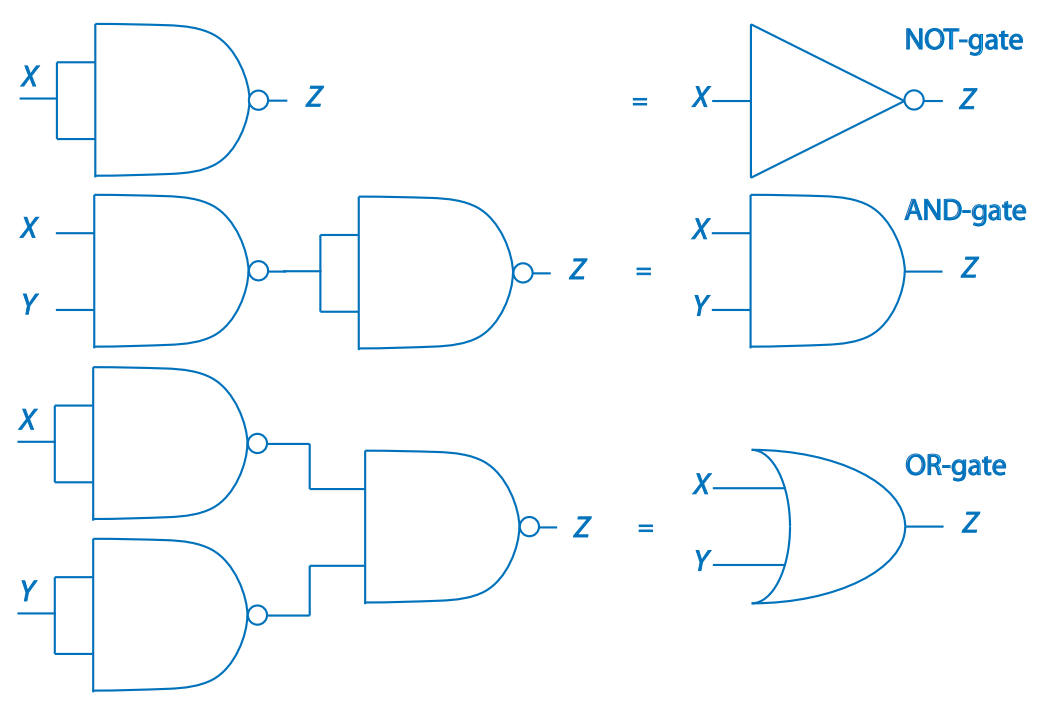
\includegraphics[width=8cm]{NAND.png}\\
\section{A binary world}
If we are given any function $f(X_1,X_2,X_3...X_N):{0,1}^n\rightarrow {0,1}$ then using AND, OR and NOT gates we can build a circuit that computes f\\
For example we can build a circuit that takes two binary inputs and outputs the addition of these two numbers\\

\begin{tabular}{lllllllll}
      & $X_3$ & $X_2$ & $X_1$ &  &   & 0 & 1 & 1 \\
      & $Y_3$ & $Y_2$ & $Y_1$ &  &   & 1 & 1 & 0 \\
      &       &       &       &  &   &   &   &   \\ \cline{1-4} \cline{6-9} 
$Z_4$ & $Z_3$ & $Z_2$ & $Z_1$ &  & 1 & 0 & 0 & 1
\end{tabular}
\\
\textbf{Half adder diagram}\\
\\
Delay in half adder from out of the not gate. May cause timing errors.\\
\\
Half adders can be combined to have more inputs, creating a full adder, the carrys connect.\\
\\
Full adders can then be connected together to give as many inputs as needed.\\
\\
Ripple adder has a cascade of full adders, need to wait for carrys from previous sum.
\section{Integrated Circuit Design not on test}
\section{Micro architecture }
\subsection{Pentium 4}
\textbf{Insert diagram from slides}\\
\\
\textbf{Datapath} - Performs the data processing operations
\begin{itemize}
\item Includes the ALU
\item A small amount of memory in the form of \textbf{registers}
\end{itemize}
\textbf{Control} - Tells the datapath, memory and I/O devices what to do\\
\textbf{Cache} - Small, fast, relatively expensive on chip memory
\subsection{von Neumann architecture}
The von Neumann arhcitecture is a fundamental computer architecture.
\begin{itemize}
\item Stored program and data both held in memory
\item Allows for self modifying programs as the processor has access to memory
\end{itemize}
The von Neumann bottleneck is the limitation of the data transfer rate between the CPU and memory. This resulted in the use of CPU caches on chip to reduce this bottleneck.\\
\\
\textbf{Harvard Architecture} - Data memory and instruction memory and separated, each with their own buses.
\subsection{Memory}
Closer it is to the CPU, the faster, but more expensive.\\
\textbf{Memory} - Pigeon holes containing data.\\
\\
Each pigeon hole has a unique address and holds 1 byte of storage.\\
\\
64 bit processors have a "word length" of 64 bits, and so can retrieve 64 bits at a time\\
\\
3 different buses:
\begin{itemize}
\item Address Bus\begin{itemize}
\item Determines location in memory
\item Width determines size of addressable memory (e.g. 4gb ram limit for 32 bit) 
\end{itemize}
\item Data Bus\begin{itemize}
\item Carries Contents of memory
\item Width determines bus size 
\end{itemize}
\end{itemize}
Comparison of different types of memory:
\begin{itemize}
\item Hard Disk - cheap to produce but slow. Permanent, so no data loss
\item RAM \begin{itemize}
\item dynamic RAM (DRAM) - data stored by transistor/capacitor, slow 
\end{itemize}
\item Cache - expensive used to store rapidly accessed data items

\end{itemize}

\section{Putting it all together}
\textbf{Register} - On chip memory locations (limited in number according to a hardware design decision) and are at the top of the memory heirarchy\\
\textbf{Accumulator} - Register that acts as a calculator
\textbf{Program counter} - Holds the address where the next instruction is found
\textbf{More from slides}\\
\\
\\
\begin{enumerate}
\item CPU outputs the value of program counter on address bus
\item 
\item Finds what instruction wants us to do
\item What data does it want to operate on
\item Look for data in memory over data bus - find what inputs needed
\item Execute the operation on the ALU
\item Answer stored in accumulator
\item Program counter updated
\item (Optional) Write the data back into memory
\end{enumerate}



\end{document}